\section{Tipologie di segnali}
Rispondiamo alla domanda più importante di questi appunti: cosa è
un segnale? Una grandezza fisica a cui associamo delle informazioni, 
quella costituisce i segnali di cui parleremo. \\
La tensione elettrica che passa ogni secondo all'interno di un circuito,
la pressione acustica esercitata sulla membrana di un microfono, perfino 
l'andamento dei titoli di una borsa, sono tutti
esempi di segnali;
matematicamente parlando possiamo paragonare un segnale ad una funzione:
un input a cui associamo delle informazioni.
\\
\\
Se consideriamo segnali in funzione del tempo, quindi grandezze fisiche che
conservono informazioni nel tempo, possiamo definire i 
\textbf{segnali determinati}. Quest'ultimi sono quei segnali che, preso 
un istante nel tempo, riusciamo a determinare l'informazione che conserva;
al contrario invece, diremo che un segnale è \textbf{aleatorio} quando non 
riuscieremo a determinare l'informazione che conserva in quel determinato
istante. \\
Di conseguenza è possibile studiare un segnale determinato tramite 
algoritmi matematici, ma lo stesso approccio non si potrà usare per 
i segnali aleatori. Data la loro naturale \emph{casuale} infatti dovremmo
usare un approccio \textbf{probabilistico}.
\\
\\
Considerando di nuovo segnali nel tempo possiamo fare un'altra distinzione
tra \textbf{segnali continui} e \textbf{segnali discreti}. \\
Molto similmente alle omonime funzioni il primo tipo indica un segnale che
è definito in ogni punto del suo \emph{intervallo}, nel secondo tipo invece 
il segnale è definito soltanto in dei \textbf{punti} del suo intervallo. 

\begin{figure}[t!]
    % --- MINIPAGE PER IL SEGNALE CONTINUO ---
    \begin{minipage}{0.48\textwidth}
        \centering
        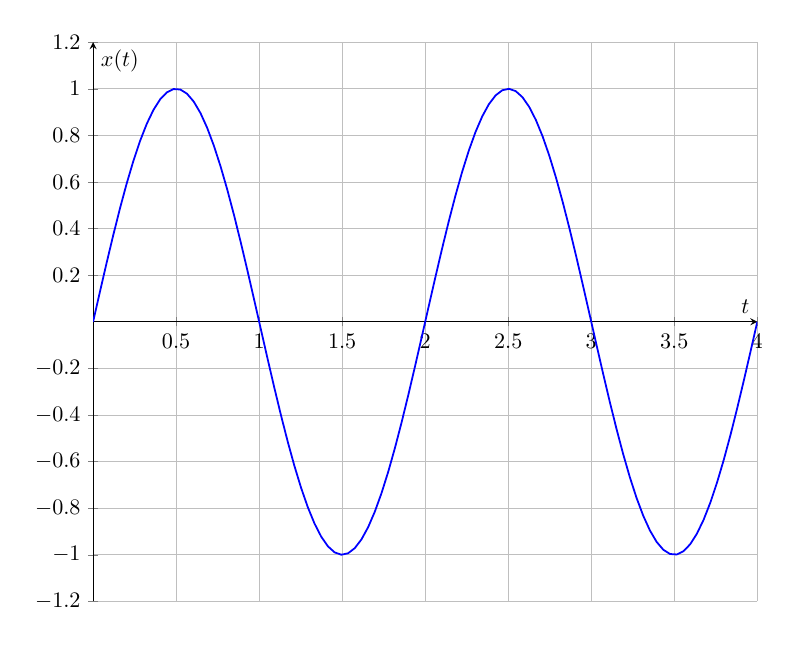
\begin{tikzpicture}[scale=0.8] % Scala leggermente per farli stare comodi
        \begin{axis}[
            axis lines = middle,
            xlabel = {$t$},
            ylabel = {$x(t)$},
            ymin = -1.2, ymax = 1.2,
            domain = 0:4,
            samples = 100,
            grid = major,
            width=\textwidth
        ]
        \addplot [blue, thick] {sin(deg(2*pi*0.5*x))};
        \end{axis}
        \end{tikzpicture}
        \caption*{Segnale a tempo continuo}
    \end{minipage}
    \hfill % Spazio elastico tra le due minipages
    % --- MINIPAGE PER IL SEGNALE DISCRETO ---
    \begin{minipage}{0.48\textwidth}
        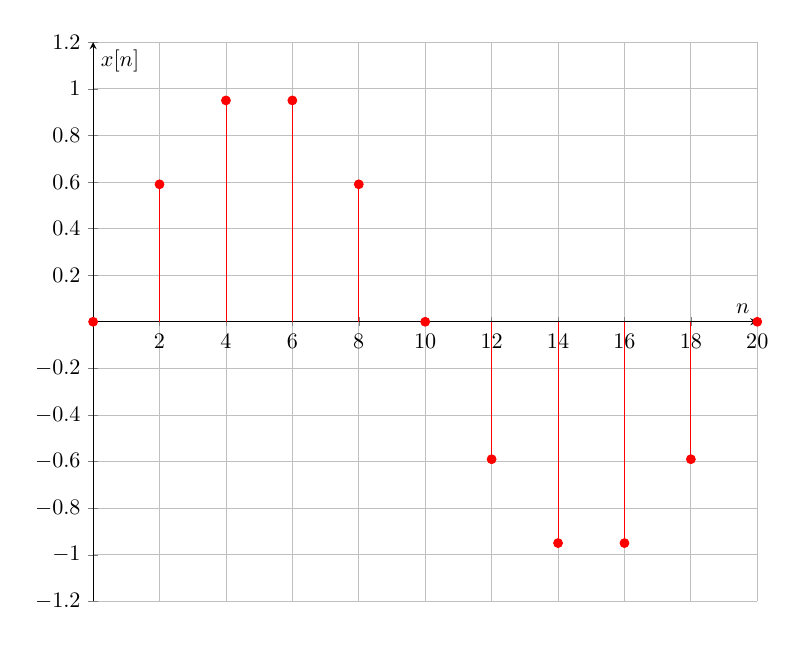
\begin{tikzpicture}[scale=0.8]
        \begin{axis}[
            axis lines = middle,
            xlabel = {$n$},
            ylabel = {$x[n]$},
            ymin = -1.2, ymax = 1.2,
            xmin = 0, xmax = 20,
            grid = major,
            width=\textwidth
        ]
        \addplot [only marks, red, mark=*] coordinates {
            (0,0) (2,0.59) (4,0.95) (6,0.95) (8,0.59) (10,0)
            (12,-0.59) (14,-0.95) (16,-0.95) (18,-0.59) (20,0)
        };
        \addplot [red, ycomb, thin] coordinates {
            (0,0) (2,0.59) (4,0.95) (6,0.95) (8,0.59) (10,0)
            (12,-0.59) (14,-0.95) (16,-0.95) (18,-0.59) (20,0)
        };
        \end{axis}
        \end{tikzpicture}
        \caption*{Segnale a tempo discreto}
    \end{minipage}
\end{figure}

\vfil

Sono gat aahah \\
Sono gat aahah \\
Sono gat aahah \\
Sono gat aahah \\
Sono gat aahah \\
Sono gat aahah \\
Sono gat aahah \\
Sono gat aahah \\
